\documentclass{beamer}
\usepackage{HECbeamer}
% \usepackage{pgfpages}
% \pgfpagesuselayout{4 on 1}[letterpaper, landscape, border shrink=5mm]
\title[\color{white}{MATH 60604A \S~5c - Model formulation}]{\texorpdfstring{MATH 60604A \\Statistical modelling \\ \S~5c - Model formulation}{MATH 60604A \\Statistical modelling \\ \S~5c - Model formulation}}
\author{Léo Belzile}
\institute{HEC Montréal\\
Department of Decision Sciences}
\date{} 

\begin{document}
\frame{\titlepage}
\begin{frame}[fragile]
\frametitle{Linear regression for the \texttt{revenge} data}
\bi
\item  Let's start by fitting an ordinary regression model, which will serve as a basis for the next analyses. 
\item This model ignores the possible within-person correlation, and proceeds as if these observations are independent.
\bi

\item  The desire for revenge for a person at a certain time is likely correlated with the desire for revenge at other times, simply because these measurements came from the same person. 
\item If this is true, the assumption that the error terms are independent is not valid; therefore, any inference made through this model is not valid.
\ei
\item The linear model is
\begin{align*}
\code{revenge} = \beta_0+\beta_1 \code{sex} + \beta_2 \code{age} + \beta_3 \code{vc} + \beta_4 \code{wom} + \beta_5 \code{t} + \varepsilon,
\end{align*}
where the error terms $\varepsilon$ are assumed independent.
\ei
\end{frame}

\begin{frame}[fragile]
\frametitle{Modelling the time effect}
\bi
\item There are two natural ways of modeling the time variable:
\bi

\item We could assume a linear effect between \code{t} and \code{revenge} (continuous variable).
\item We could instead include \code{t} as a categorical variable.
\ei

\item  We will use \code{proc mixed} in order to familiarize you with this procedure.
 \ei

\begin{tcolorbox}[colback=white, colframe=hecblue, title=\SASlang{} code to fit a linear model]
\begin{verbatim}
proc mixed data=statmod.revenge method=reml;
model revenge = sex age vc wom t / solution;
run;
\end{verbatim}
\end{tcolorbox}
\end{frame}
 \begin{frame}
\frametitle{\code{proc mixed} output for linear regression}
\begin{center}
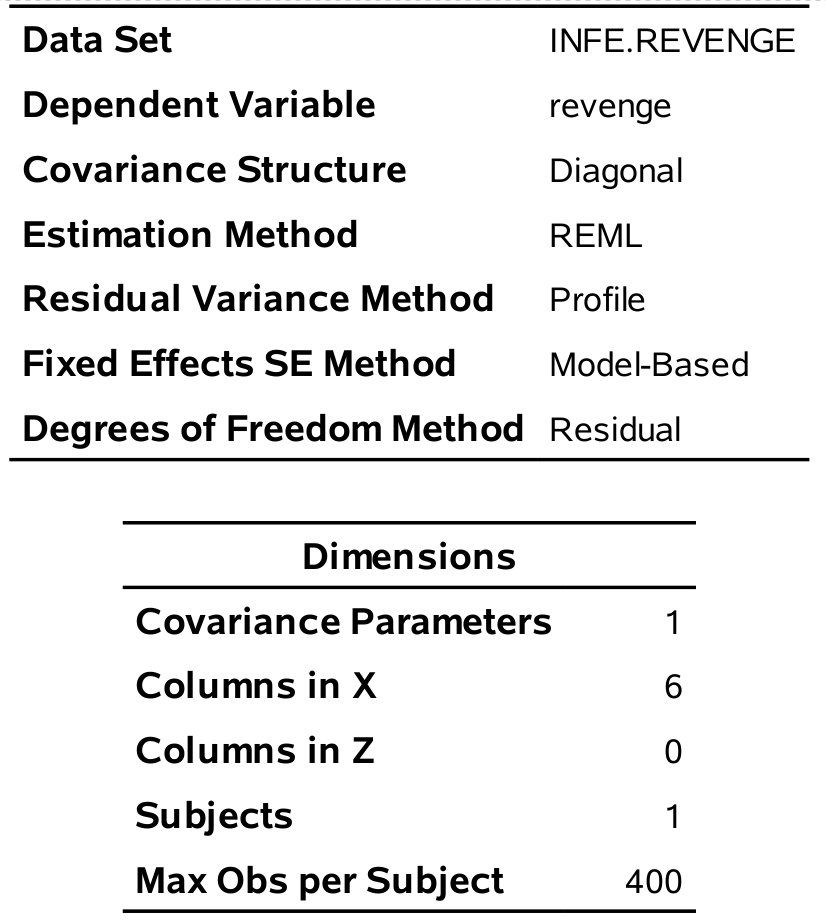
\includegraphics[width = 0.45\linewidth]{img/c5/slides6-e03}
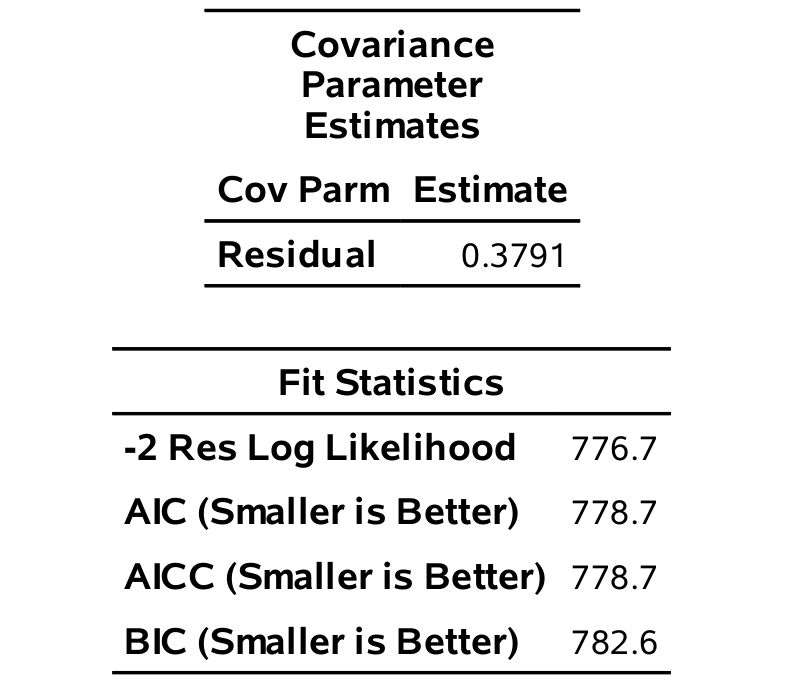
\includegraphics[width = 0.45\linewidth]{img/c5/slides6-e04}
\end{center}
{\footnotesize
The output of \code{proc mixed} is more complicated than that of \code{proc glm}. 


}
\end{frame}

 \begin{frame}
\frametitle{Mean parameter estimates}
\begin{center}
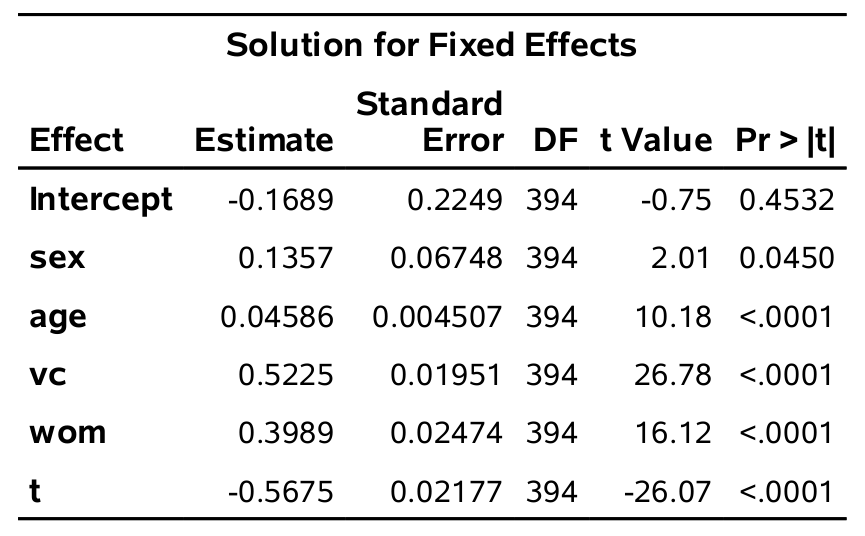
\includegraphics[width = 0.7\linewidth]{img/c5/slides6-e05}
\end{center}
We see that all the variables are significant, though just barely for \code{sex}.
\end{frame}

 \begin{frame}
\frametitle{Interpretation of parameters for linear regression}
\bi
\item The more the person had initial behaviour of type \code{vc} or \code{wom}, the higher the desire for revenge. 
\item The effect of time is particularly interesting here. We see that the effect is negative. In each questionnaire, the value of \code{revenge} decreases by $0.568$, on average, when all other variables remain constant. This is exactly what we saw in our earlier plots.
\item \alert{But can we be confident in our hypothesis tests?} The answer is no. Any kind of inference (tests and confidence intervals) will not be valid when we ignore the within-person correlation.
\ei
\end{frame}


\section{Linear model with correlated errors}


\begin{frame}
\frametitle{Notation}
\bi
\item Suppose that we collect observations from $m$ groups such that:
\be
\item There are $n_i$ observations within group $i$ ($i=1, \ldots, m$).
\item Any two observations from the same group are possibly correlated.
\item Any two observations from different groups are assumed independent.
\ee
\item Groups can be formed in several ways:
\bi

\item Several measures can be taken from the same subject (repeated measures) and each individual forms a group. 
\item A group could also consist of individuals from the same school, department, or family.
\ei
\item As before, we assume that we have a response variable
 and a collection of $p$ explanatory variables.
\item To simplify the notation, we'll call $\mathbf{X}_i$ the set of all explanatory variables for all observations in group $i$.

\ei
\end{frame}


\begin{frame}
\frametitle{Notation}
\bi
\item We use the index $i$ to indicate the group, and $j$ to indicate an observation within a group.
\bi

\item If the group is a business, then $i$ represents the business, and $j$ represents the subject.
\item For longitudinal data, $i$ represents the subject and $j$ represents an observation for that subject at a specific \textbf{time}.
\ei
\item We call $\bs{Y}_i=(Y_{i1}, \ldots, Y_{in_i})$ the \alert{set of observations} of the outcome variable for group $i$. 
\item For the explanatory variables, we now need three indices, namely 
\bi \item $i$ for the group,
\item $j$ for the observation number within the group
\item $k$ for the explanatory variable.
\ei
\item We call  $\mathbf{X}_{ij}=(1, \mathrm{X}_{ij1}, \ldots, \mathrm{X}_{ijp})$ the set of $p$ explanatory variables for observation $j$ in group $i$.

\ei
\end{frame}

\begin{frame}
\frametitle{Linear model with correlated errors}
The linear regression model is
\begin{align*}
Y_{ij}=\beta_0+\beta_1\mathrm{X}_{ij1}+\cdots+\beta_p \mathrm{X}_{ijp}+\varepsilon_{ij}
\end{align*}
for $i=1, \ldots, m$ and $j=1, \ldots, n_i$, where $\varepsilon_{ij}$ is the error term for observation $j$ in group $i$.
\bi
\item As before, we assume that $\E{\varepsilon_{ij}\mid  \mathbf{X}_{ij}}=0$ and therefore
\begin{align*}
\E{Y_{ij}\mid \mathbf{X}_i}=\beta_0+\beta_1\mathrm{X}_{ij1}+\cdots+\beta_p \mathrm{X}_{ijp}. 
\end{align*}
% \item We still assume constant variance for the error terms; that is, $\Va{\varepsilon_{ij}}=\sigma^2$.
% \item However, \alert{we no longer assume that the error terms are independent}.
\ei
\end{frame}



\begin{frame}
\frametitle{Covariance/correlation structure}
\bi
\item When we assume that the $\mathbf{X}$ terms are fixed, correlation between error terms $\bs{\varepsilon}$ is equivalent to correlation among the responses $\bs{Y}$.
\item We will allow dependence  between observations within the same group. 
\item We assume the groups are independent from one another, so $\Co{\eps_{ij},\eps_{i'j'}}=0$ if $i \neq i'$.
\item We model the \alert{within-group} correlation by assuming that the covariance matrix of $\bs{Y}$ for group $i$ is
\begin{align*}
\Co{\bs{Y}_i\mid \mathbf{X}_i}=\bs{\Sigma}_i,
\shortintertext{
or equivalently}
\Co{\bs{\varepsilon}_i\mid \mathbf{X}_i}=\bs{\Sigma}_i,
\end{align*}
where $\bs{\varepsilon}_i=(\varepsilon_{i1}, \ldots, \varepsilon_{in_i})$ is the vector of errors for group $i$.
\ei
\end{frame}




\begin{frame}
\frametitle{Block covariance structure for longitudinal data}
\bi 
\item 
Assume for simplicity that data are ordered by group.
 \item We assume that observations for group  $i$ are correlated, but the observations for different groups are independent.
 \item 
  The full covariance matrix of the \textbf{measurements} is therefore \textbf{block-diagonal}, i.e.,
 \begin{align*}
  \Co{\bs{Y}} = \begin{pmatrix}
                 \bs{\Sigma}_1 & \mathbf{O} & \cdots & \mathbf{O}\\
                  \mathbf{O} &\bs{\Sigma}_2 & \cdots & \mathbf{O} \\
                  \vdots & \ddots & \ddots & \vdots \\
                   \mathbf{O} & \mathbf{O} & \cdots & \bs{\Sigma}_m 
                \end{pmatrix}.
\end{align*}
\bi 
\item In our \texttt{revenge} example, we have $n=80 \times 5 = 400$ observations.
\item The \alert{within-group covariance} matrix, $\bs{\Sigma}_i$, is $5 \times 5$ because we have a balanced sample ($n_1 = \cdots = n_m=5$). The block $\bs{\Sigma}_i$ is thus identical for each group.
\item The \textbf{between-group} covariance is \textbf{zero} ($\mathbf{O}$) because we assumed data for different individuals are independent from one another.
\ei
\ei
\end{frame}



\begin{frame}
\frametitle{Covariance/correlation structure}
\bi
\item Generally, the covariance structure will depend on several parameters that will be estimated at the same time as the $\bs{\beta}$ parameters. 
\item The covariance structure is specified by the analyst. Sometimes, several covariance structures can be fitted to see which is most appropriate for the data at hand. 
\ei
\end{frame}

\end{document}
